%!TEX program = lualatex
%!TEX encoding = UTF-8 Unicode  
%!TEX root = chapter01.tex  
\documentclass[main.tex]{subfiles} 
\begin{document} 
	%----------------------------------------------------------------------------------------
%	CHAPTER 1
%----------------------------------------------------------------------------------------
\cleardoublepage 
\loadgeometry{marginlayout}  
\pagestyle{scrheadings} % Print headers again  
\KOMAoptions{
	headwidth=textwithmarginpar,
	headsepline=true,
	headsepline= 0.5pt,
	footwidth=textwithmarginpar,
}   
\onehalfspacing 
\chapter{Arithmétique. Nombres entiers}


%----------------------------------------------------------------------------------------
%	 
%----------------------------------------------------------------------------------------

%Nombres entiers, fractions
%Déterminer les diviseurs d’un nombre entier.
%Utiliser les critères de divisibilité par 2, 3, 5, 9 et 10.
%Connaître la liste des nombres premiers inférieurs ou égaux à 30.
%Prouver qu’un nombre est premier.
%Décomposer un nombre entier en produit de facteurs premiers.
%Modéliser et résoudre des problèmes mettant en jeu la divisibilité.
%Connaître et utiliser un tableur, lire et exécuter un programme sur Scratch.
%----------------------------------------------------------------------------------------
%	 
%----------------------------------------------------------------------------------------


\section{Arithmétique sur les nombres relatifs}
Entrainement \url{http://mathsmentales.net/}
\begin{itemize}
	\item  addition de relatifs \url{http://bref.jeduque.net/hd71fr}
	\item  soustraction de relatifs \url{http://bref.jeduque.net/dnpufe}
	\item  multiplication de relatifs \url{http://bref.jeduque.net/fhxet7}, 3 relatifs \url{http://bref.jeduque.net/jbk1tp}
	\item  quotient de relatifs \url{http://bref.jeduque.net/7rcvbu} 
\end{itemize}

%----------------------------------------------------------------------------------------
%	 
%----------------------------------------------------------------------------------------

\newpage 
\loadgeometry{marginlayout}  
\pagestyle{scrheadings} % Print headers again  
\KOMAoptions{
	headwidth=textwithmarginpar,
	headsepline=true,
	headsepline= 0.5pt,
	footwidth=textwithmarginpar,
} 
\onehalfspacing
\section{Facteurs, multiples et division euclidienne}
\begin{definition}[Multiples]
	Soit deux entiers $n$ et $m$.
	
	$m$ est un multiple de $n$ \textbf{si et seulement si} il existe un entier $k$ tel que $m=k\times n$.
	
	Les multiples de $n$ tous les nombres de la forme $kn$, où $k$ est un entier.
\end{definition}
\begin{example}\hfill 
	\begin{enumerate}[label={\alph*)}, leftmargin=*]  
		\item $45$ est un multiple de $9$ et de $5$ car $45=5\times 9$.  
		\item Enumérer tous les diviseurs de $45$. 
	\end{enumerate}
\end{example}
\begin{remark}
	Pour tout $m\in \mathbb{N}$,  $0=0\times m$. Donc  \textbf{$0$ est un multiple de tout entier, et tout entier divise $0$}. Néanmoins, l'usage est souvent d'ignorer $0$ comme multiple. 
\end{remark}
\begin{definition}[Division entière] Soit les entiers $n$ et $d$ ($d\neq 0$).
	
	On appelle quotient de $n$ par $d$ l'entier $q$ tel que : 
	\[ qd\leqslant n < qd + d\]
	
	Le reste de la division de $n$ par $d$  est l'entier définit par :
	\[ n = qd + r
	\qquad 0\leqslant r < d \]
	
	$n$ est un multiple de $d$ s.s.i. le reste de la division de $n$
	par $d$ est nul.
\end{definition}
\begin{example} 
	\begin{marginfigure} [-2cm]
		\opidiv[displayintermediary=all,voperation=top]{17}{5}\hfill 
		\opidiv[displayintermediary=all,voperation=top]{20}{5}
		\caption{$17=3\times 5 + 2$ et $20 = 4 \times 5$}
		\label{chapitre03:figure:divisionentiere}
	\end{marginfigure}
	\begin{enumerate}[label={\alph*)}, leftmargin=*]  
		\item $3\times 5\leqslant 17<4\times 5$ et $17=3\times 5+2$. 
		\item $4\times 5\leqslant 20<5\times 5$ et $20=4\times 5+0$.  
	\end{enumerate} 
\end{example}

\begin{marginfigure}
	\begin{scratch}[scale=0.8, num blocks=true]
		\blockif{si \booloperator{ \ovaloperator{\ovalvariable{nbr} modulo \ovalvariable{7}} = \ovalnum{0}}}
		{ 
			\blocklook{dire \ovalnum{VRAI}}  
		} 
	\end{scratch}
	\caption{Un script pour tester si nbr est divisible par 7} 
\end{marginfigure} 


\begin{remark} Dans \texttt{Scratch}, l'instruction \ovaloperator{\ovalvariable{$n$}~modulo~\ovalvariable{$d$}} permet de calculer le reste de la division de \ovalvariable{$n$} par \ovalvariable{$d$}.
	
	Par exemple \ovaloperator{\ovalnum{12}~modulo~\ovalnum{5}}=2.
\end{remark} 
\begin{remark} La touche {\fontspec{CASIO ClassWiz Fr}-} permet de calculer le quotient et le reste d'une division euclidienne.
	\end{remark}
%----------------------------------------------------------------------------------------
%	EXERCICES
%----------------------------------------------------------------------------------------

\newpage 
\loadgeometry{widelayout}  
\pagestyle{scrheadings} % Print headers again  
\KOMAoptions{
	headwidth=textwithmarginpar,
	headsepline=true,
	headsepline= 0.5pt,
	footwidth=textwithmarginpar,
} 
\onehalfspacing
\subsection{Exercices}

\begin{exercise}\hfill 
\begin{enumerate}[label={\alph*)},    leftmargin=*] 
	\item Le plus grand reste possible dans une division euclidienne par 54 est \BoiteFlash{}.
	\item On a $\numprint{92947}=9\times\numprint{10327}  + 4$\\
		Écrire le quotient et le reste de la division euclidienne de \numprint{92947} par 9.
		\item Les trois divisions euclidiennes suivantes sont exactes : \\
		$\numprint{4545} = 102 \times 44 + 57$\hfill 
		$\numprint{4545} = 100 \times 45 + 45$\hfill 
		$\numprint{4545} = 101 \times 45 + 0$ \hfill\null 
		 
		Sans calculer, dire si les nombres 102; 100; 101 sont des diviseurs de \numprint{4545}. Justifier.
		\item Avec la calculatrice, compléter chaque phrase avec \og est un diviseur de\fg{} ou \og est un multiple de\fg{} ou \og n'est ni un diviseur ni un multiple de \fg{} :
		\begin{multicols}{2}
		229 \BoiteFlash{\rule{0cm}{1.6em}\rule{5cm}{0em}} \numprint{1832}\\
		689 \BoiteFlash{\rule{0cm}{1.6em}\rule{5cm}{0em}}  539\\
		455 \BoiteFlash{\rule{0cm}{1.6em}\rule{5cm}{0em}}  179\\
		\numprint{2391} \BoiteFlash{\rule{0cm}{1.6em}\rule{5cm}{0em}}  797\\
		\;\;\;41 \BoiteFlash{\rule{0cm}{1.6em}\rule{5cm}{0em}}  164\\
		\;\;687 \BoiteFlash{\rule{0cm}{1.6em}\rule{5cm}{0em}} 229
		\end{multicols}
\end{enumerate}
\end{exercise} 
\begin{exercise}[sommes de contrôle] \hfill 
	
	Le  numéro de série horizontal sur le dos d'un billet de monnaie authentique vérifie la propriété suivante  \og la somme du nombre de lettres, du rang de chaque lettre dans l'alphabet et des chiffres est divisible par 9\fg{}.
	\begin{enumerate} [label={\alph*)},    leftmargin=*] 
		\item Vérifier que les numéros de série suivants semblent correct : U13056999935, VA7599836405.%, ZC2664133259. 
		\item Sur un billet authentique, figure le numéro S0216644810-. Le dernier chiffre est illisible, retrouvez-le.
		\item Sur un autre billet authentique, on lit -16122340242. La lettre est effacée. Quelles sont les lettres possibles ?
	\end{enumerate}
\end{exercise}
\medskip
\begin{exercise}\hfill 
	
	 En utilisant les critères de divisibilité  indiquer si l'on peut simplifier chaque fraction par $2$, $3$, $4$, $5$, $9$ ou $10$ :
	
\noindent\parbox{0.5\linewidth}{
\QCM[Multiple,Alterne,Reponses=6,Stretch=1.2,Largeur=0.5cm,%
Noms={{$2$}/{$3$}/{$4$}/{$5$}/{$9$}/{$10$}}]{%\textbb{N} marche pas{$2$}/{$3$}/{$4$}/{$5$}/{$9$}/{$10$}
	{$\tfrac{45}{30}$}&0&1&0&1&0&0, 
	{$\tfrac{54}{81}$}&0&1&0&0&1&0, 
	{$\tfrac{1557}{1341}$}&0&1&0&0&1&0, 
} 
}\hfill \parbox{0.5\linewidth}{
\QCM[Multiple,Alterne,Reponses=6,Stretch=1.2,Largeur=0.5cm,Depart=4,%
Noms={{$2$}/{$3$}/{$4$}/{$5$}/{$9$}/{$10$}}]{%\textbb{N} marche pas{$2$}/{$3$}/{$4$}/{$5$}/{$9$}/{$10$}  
	{$\tfrac{4962}{11334}$}&1&1&0&0&0&0,  
	{$\tfrac{2034}{6066}$}&1&1&0&0&1&0, 
	{$\tfrac{1460}{2180}$}&1&0&1&1&0&1, 
} 
}

\end{exercise} 
\medskip
\begin{exercise}\hfill 
	
\noindent	Léa a travaillé pendant les vacances scolaires et a touché son premier salaire.
	Deviner son salaire sachant que c’est un nombre entier entre 500 et 700 euros, multiple de 9 et de 10 et divisible par 4. 
	Expliquer la réponse.
\end{exercise}

\newpage 
\begin{example}Écrire la liste de tous les diviseurs de $36$ et $60$.  On teste la divisibilité par 1, puis 2, puis 3, puis 4 , etc.   
	\begin{align*} 
		36 & =1\times 36 & 60 &= 1\times 60\\
		&= 2\times 18 & 60 &=\\
		&= 3\times 12 & 60 &=\\
		&= 6\times 6 & 60 &=\\
		&= 12\times 3 & 60 &=\\
		&= 18\times 2 & 60 &=\\
		& = 36 \times 1 &60 &= \sqrt{60}\times  \sqrt{60}
	\end{align*} 
 $\operatorname{Diviseurs}(36)=\{ 1; 2; 3; 6; 12; 18; 36\}$
\end{example}
\medskip
\begin{exercise} \hfill 
	\begin{enumerate} [label={\alph*)},    leftmargin=*] 
		\item Écrire la liste de tous les diviseurs de  $92$, $56$, $12$ et $30$.
		\item Quel est le plus grand diviseur commun à $92$ et $56$ ? Même question pour $12$ et $30$. 
		\item Écrire les fractions $\frac{92}{56}$ et $\frac{12}{30}$ sous forme irréductible.
	\end{enumerate}
\end{exercise} 
\medskip
 \begin{exercise}[un classique]  \hfill 
 	
 \noindent	On souhaite repartir 42 filles et 90 garçons en des équipes qui contiennent le même nombre de filles et le même nombre de garçons. 
 	\begin{enumerate}[label={\alph*)},    leftmargin=*] 
 		\item Peut-on les repartir sur 5 équipes ? Justifier.
 		\item Écrire la liste des diviseurs de 42 et 90.
 		\item Quel est le plus grand nombre d'équipes réalisable ?
 	\end{enumerate} 
 \end{exercise}
\medskip
 \begin{exercise} \hfill 
 	
 \noindent	Un fleuriste dispose de 126 iris et 210 roses.
 	Il veut en utilisant toutes ses fleurs, réaliser des bouquets contenant tous le même   nombre d’iris et le même nombre de roses.
 	\begin{enumerate}[label={\alph*)},    leftmargin=*] 
 		\item Le fleuriste peut-il réaliser 15 bouquets ?
 		\item  Peut-il réaliser 14 bouquets ? 
		\item   Quel nombre maximal de bouquets peut-il réaliser ?
		\item    Donner la composition de chacun d’eux ? 
 	\end{enumerate}  
 \end{exercise} 
\medskip
\begin{exercise}\hfill %\label{BB01.exo.04}\hfill \textbf{16 points} %20min 
	
	\noindent Carole souhaite réaliser une mosaïque sur un mur de sa maison. La surface à paver est un
	rectangle de dimensions \SI{108}{\centi\meter}  et  \SI{225}{\centi\meter}  et doit être entièrement recouverte par des carreaux de faïence carrés de même dimension sans découpe. 
	\begin{enumerate}[label={\alph*)},    leftmargin=*] 
		\item Carole peut-elle utiliser des carreaux de \SI{3}{\centi\meter}  de côté ? De \SI{6}{\centi\meter}  de côté ?
		\item Quelle est la dimension maximale des carreaux que Carole peut poser ?
		
		Combien de carreaux utilisera-t-elle ?
	\end{enumerate}
\end{exercise}
\begin{example}[Illustration géométrique de l'algorithme d'Euclide \url{https://www.geogebra.org/m/qjd4ngam}] \hfill 
	
	\noindent\parbox[position=t]{0.45\linewidth}{  \centering
	\begin{tikzpicture}[scale=1.0] 
		\tkzInit[ xstep=50, ystep=50]
		\tkzSetUpPoint[size=3, fill=black]
		\tkzfctset{tan style/.style={->,>=latex, color=red, line width=1.2pt}}   
		\tkzSetUpLine[line width= 1.2pt, add=.5 and .5] 
		
		
		\def \a{345};
		\def \b{150};
		\pgfmathparse{int(\a/\b)}
		\edef\c{\pgfmathresult};
		 
		\tkzDefPoint(0,0){A} 
		\tkzDefPoint(\a,0){B} 
		\tkzDefPoint(\a,\b){C} 
		\tkzDefPoint(0,\b){D} 
		\tkzDrawPolygon[](A,B,C,D)
		\foreach \i in {0,1,...,{\c}}{% 
			\tkzDefPoint({\i*\b},0){E}
			\tkzDefPoint({\i*\b},\b){F} 
			\tkzDrawSegments(E,F)
		}
	
	
		\pgfmathparse{int(\a-\c*\b)}
		\edef \d{\pgfmathresult};
		\pgfmathparse{int(\a-\d)}
		\edef \e{\pgfmathresult}; 
		\pgfmathparse{int(\b/\d)}
		\edef \f{\pgfmathresult};
%		\tkzDefPoint({\a-\d},{\d}){G} 
%		\tkzDefPoint({\a},{\d}){H} 
%		\tkzDrawSegments(G,H)	 
		\foreach \i in {0,...,\f}{% 
			\tkzDefPoint(\e,{\i*\d}){G} 
			\tkzDefPoint(\a,{\i*\d}){H} 
			\tkzDrawSegments(G,H)
		} 

%		\tkzDefPoint(1,0){E}
%		\tkzDefPoint(1,-1){F}
%		
%		\tkzDefPoint(2,0){G}
%		\tkzDefPoint(2,-1){H}
%		
%		\tkzDefPoint(2,2-5**0.5){I}
%		\tkzDefPoint(5**0.5,2-5**0.5){J}
%		
		\tkzDrawSegment[dim={\scriptsize ${\a}$,-15pt,}](A,B)
		\tkzDrawSegment[dim={\scriptsize ${\b}$,+15pt,}](A,D)
%		\tkzDrawSegments[dashed](E,F G,H)
%		\tkzDrawPolygon[fill=gray!20](I,J,C,H)  
%		\tkzLabelPoint[above left](A){\scriptsize$A$}
%		\tkzLabelPoint[above right](B){\scriptsize$B$} 
%		\tkzLabelPoint[below right](C){\scriptsize$C$} 	
%		\tkzLabelPoint[below](D){\scriptsize$D$} 
%		\tkzLabelPoint[above](E){\scriptsize$E$} 
%		\tkzLabelPoint[below](F){\scriptsize$F$} 
%		\tkzLabelPoint[above](G){\scriptsize$G$} 
%		\tkzLabelPoint[below](H){\scriptsize$H$}  
%		\tkzLabelPoint[left](I){\scriptsize$I$} 
%		\tkzLabelPoint[right](J){\scriptsize$J$} 
	\end{tikzpicture}
}\hfill 
\parbox[position=r]{0.5 \linewidth}{    
À chaque étape, on remplit le rectangle restant par des carrés de côté égal à la longueur du plus petit côté.

\opidiv[style=text]{345}{150} ; 
%\hfill $\operatorname{PGCD}(345;150)=\operatorname{PGCD}(264;228)$.

\opidiv[style=text]{150}{45} ;  

\opidiv[style=text]{45}{15} ;  
}  
\end{example}

\begin{exercise}[\url{https://link.dgpad.net/d9zJ}]\hfill 
	
\noindent\parbox{0.4\linewidth}{
\begin{scratch}[scale=0.95,num blocks=true,print, fill blocks, fill gray=0.95]
%	\blockinit{quand \greenflag est cliqué} 
%	\blocksensing{demander \ovalnum{saisir un entier} et attendre}
%	\blockvariable{mettre \selectmenu{a} à \ovalsensing{réponse}}
%	\blocksensing{demander \ovalnum{saisir un entier} et attendre}
%	\blockvariable{mettre \selectmenu{b} à \ovalsensing{réponse}}
	\blockvariable{mettre \selectmenu{a} à \ovalvariable{\rule{0cm}{1.0em}\rule{1.5cm}{0em}}} 
	\blockvariable{mettre \selectmenu{b} à \ovalvariable{\rule{0cm}{1.0em}\rule{1.5cm}{0em}}} 
	\blockvariable{mettre \selectmenu{r} à \ovaloperator{\ovalvariable{a} modulo \ovalvariable{b}}}
	\blockrepeat{répéter jusqu'à ce que \booloperator{ \ovalvariable{r} = \ovalnum{0}}}
	{
		\blockvariable{mettre \selectmenu{a} à \ovalvariable{b}}
		\blockvariable{mettre \selectmenu{b} à \ovalvariable{r}}
		\blockvariable{mettre \selectmenu{r} à \ovaloperator{\ovalvariable{a} modulo \ovalvariable{b}}}	
	}
	\blocklook{dire \ovalvariable{b} pendant \ovalnum{$5$} secondes} 
\end{scratch}
}\hfill 
\parbox{0.55\linewidth}{
On saisit les valeur $\ovalvariable{a}=42588$ et $\ovalvariable{b}=276822$.
\begin{enumerate}[label={\alph*)},    leftmargin=*] 
	\item   Faire tourner à la main le script ci-contre et remplir le tableau ci-dessous. Quel est le nombre de répétition de la boucle ?
	
\begin{tabularx}{0.95\linewidth}{|c|X|X|X|}\hline 
	& \ovalvariable{a} &\ovalvariable{b} &\ovalvariable{r} \\ \hline
avant la ligne 4 & && \\ \hline
après 1 boucle &&& \\\hline 
après 2 boucles &&& \\ \hline
après 3 boucles &&& \\\hline
après 4 boucles &&& \\ \hline 
après 5 boucles &&& \\ \hline 
\end{tabularx} 
	\item Rendre irréductible la fraction $\frac{42588}{276822}$. 
	\item Préciser ce qu'affiche le programme pour $\ovalvariable{a}=23$ et $\ovalvariable{b}=42$. Que peut-on en déduire de la fraction $\frac{23}{42}$ ?
\end{enumerate}   
}
	\end{exercise}
 
 \begin{exercise}  \hfill 
 	
 \noindent	Un chocolatier a fabriqué 108  pralines et 135 chocolats. Il souhaite constituer les ballotains ainsi :
 	\begin{itemize}
 		\item le nombre de pralines est le même dans chaque ballotins ;
 		\item le nombre de chocolats est le même dans chaque ballotins ;
 		\item tous les chocolats et toutes les pralines sont utilisés.
 	\end{itemize} 
 	\begin{enumerate}[label={\alph*)},    leftmargin=*] 
 		\item Peut-il utiliser exactement 9 ballotins ?  12 ballontins ?
 		\item Quel nombre maximal de ballotins pourra-t-il réaliser ?
 		\item Combien y aura-t-il alors de chocolats et de pralines dans chaque ballotins ?
 		\item Une entreprise souhaite lui acheter ces boîtes. Compléter la facture ci-dessous :
 		
 \begin{table*}[h]
 	\begin{tabularx}{1\columnwidth}{|X|c|c|c|c|c|}\hline 
 		\rule{0pt}{1.8em}Produit & Quantité & Prix unitaire HT & Montant HT& Montant TVA \numprint{5.5}~\% & Montant TTC \\ \hline
 		Ballotin Choco-praline & 20 & \EUR{7.80}&&&\\\hline 
 		\end{tabularx}
 \end{table*}
 	\end{enumerate}  
 \end{exercise} 
 
\begin{exercise} 
Analyser les deux scripts ci-dessous  et décrire ce que représente la variable \ovalvariable{a} pour \ovalnum{108} en fin de chaque script.
 
\noindent\parbox{0.45\linewidth}{
	\begin{scratch}[scale=0.8 ,num blocks=true,print, fill blocks, fill gray=0.95] 
		\blockvariable{mettre \selectmenu{a} à \ovalnum{0} } 
		\blockvariable{mettre \selectmenu{b} à \ovalnum{1} } 
		\blockrepeat{répéter  \ovalnum{108} fois}
		{ 
			\blockif{si \booloperator{ \ovaloperator{\ovalvariable{b} modulo \ovalnum{9}} = \ovalnum{0}} alors}
			{\blockvariable{ajouter \ovalnum{1} à \selectmenu{a}}}
			\blockvariable{mettre \selectmenu{b} à \ovaloperator{\ovalvariable{b} $+$ \ovalvariable{1}}}		 
		}
	\end{scratch}
}\hfill
\parbox{0.45\linewidth}{
	\begin{scratch}[scale=0.8 ,num blocks=true,print, fill blocks, fill gray=0.95] 
		\blockvariable{mettre \selectmenu{a} à \ovalnum{0} } 
		\blockvariable{mettre \selectmenu{b} à \ovalnum{1} } 
		\blockrepeat{répéter  \ovalnum{108} fois}
	{ 
		\blockif{si \booloperator{ \ovaloperator{\ovalnum{108} modulo \ovalvariable{b}} = \ovalnum{0}} alors}
			{\blockvariable{ajouter \ovalnum{1} à \selectmenu{a}}}
		\blockvariable{mettre \selectmenu{b} à \ovaloperator{\ovalvariable{b} $+$ \ovalvariable{1}}}		 
	}
\end{scratch}
} 
\end{exercise}


\begin{exercise}\hfill 
	
	Effectuer les calculs suivant et donner les résultats sous forme de fraction irréductible. Détailler les étapes pour ramener au même dénominateur.
	\begin{multicols}{3}
		\begin{enumerate}[label={$\alph*=$\rule{0pt}{1.6em}}]
			\item $2+\frac{7}{-30}$
			\item $3+\frac{-7}{5}$
			\item $\frac{1}{15}-\frac{4}{5}-2$ 
			\item $\frac{5}{7}-\frac{2}{7}\times \frac{4}{3}$
			\item $\frac{7}{12}-\frac{1}{8}$
			\item $\frac{7}{6}+\frac{7}{16}$
			\item $\frac{3}{20}+\frac{4}{25}$
			\item$\frac{2}{7}+\frac{5}{21}$
			\item$\frac{7}{12}+\frac{5}{18}-\frac{3}{4}$
		\end{enumerate}
	\end{multicols} 
\end{exercise} 

 \begin{exercise} \hfill 
 	
 	\begin{figure*}[h]
 	\begin{tikzpicture}
 		\tkzSetUpPoint[size=3, fill=black]
 		\tkzfctset{tan style/.style={->,>=latex, color=red, line width=1.2pt}} 
 		\tkzDefPoint(0,0){A}
 		\tkzDefPoint(4,0){B} 
 		\tkzDrawLine[add=.2 and 1](A,B)
 		
 		\tkzDefPoint(0,2.5){C}
 		\tkzDefPoint(0,-1.3){D}
 		\tkzDrawCircle[diameter](A,C)
 		
 		\tkzDrawCircle[diameter](A,D)
 		
 		\tkzDrawPoints(A)
 		\tkzLabelPoint[above](A){$A$}
 	\end{tikzpicture}
 \end{figure*}
 On fait rouler deux cercles de périmètre 42\si{\centi\meter} et 8\si{\centi\meter} le long d'une ligne horizontale. On marque les 2 cercles en un point A. Au début les deux marques sont en contact.
 \begin{enumerate}[label={\alph*)},    leftmargin=*] 
 	\item Après combien de tours pour chaque cercle, les marques sont à nouveau en contact ?
 	\item Même question pour des cercles de perimètre 12\si{\centi\meter} et 18\si{\centi\meter}.
 \end{enumerate}
\end{exercise}
\begin{exercise}\hfill 

Deux ampoules clignotent. L’une s’allume toutes les 153 secondes et l’autre toutes les
187 secondes. À minuit, elles s’allument ensemble.
Détermine l’heure à laquelle elles s’allumeront de nouveau ensemble.
\end{exercise} 
%----------------------------------------------------------------------------------------
%	 
%----------------------------------------------------------------------------------------

\newpage 
\loadgeometry{marginlayout}  
\pagestyle{scrheadings} % Print headers again  
\KOMAoptions{
	headwidth=textwithmarginpar,
	headsepline=true,
	headsepline= 0.5pt,
	footwidth=textwithmarginpar,
} 
\onehalfspacing 
\section{Nombres premiers}
\begin{definition}
	Un nombre entier est \textbf{premiers} s'il admet \textbf{exactement} 2 diviseurs \textbf{différents} : 1 et lui même.
\end{definition}
On classe les nombres entiers positifs en 3 catégories :
\begin{description}
	\item[l'unité] 1
	\item[les nombres premiers] 2, 3, 5...
	\item[les nombres composés] tout le reste.
\end{description}
\begin{theorem}[Nombres premiers < 100]   sont :
	\begin{enumerate}[label=\textbullet, leftmargin=*]
		\item $2$, $3$, $5$ et $7$.
		\item tous les nombres non divisibles par 2, 3, 5 et 7.
	\end{enumerate}
\end{theorem}
\begin{example}
	$11$ , $31$ et $97$ sont des nombres premiers.
\end{example} 
\begin{theorem}[Test de primalité (admis)]  
	Si $n\in\mathbb{N}^*$ n'admet pour diviseur aucun des nombres (premiers) compris entre 2 et $\sqrt{n}$, alors $n$ est premier.
\end{theorem}
\begin{example}
	Vérifier que les nombres $149$ et $173$ sont premiers.
\end{example}

\begin{theorem}[théorème fondamental de l'arithmétique]  Tout nombre entier $n\in\mathbb{N}^*$ se décompose de manière unique (à l'ordre près) en produit de  facteurs premiers.
\end{theorem}
\begin{example}
	$31$ est un nombre premier, sa décomposition en facteurs premiers est lui-même.
	
	$1008=2^4\times 3^2 \times 7^1$. Le facteur 2 a pour multiplicité 4.
	
	$25777=149\times 173$.
\end{example} 
\begin{marginfigure}
\begin{tikzpicture}[scale=1] 
	\node[inner sep=0pt, opacity=1] (carte) at (0,0) {
		\includegraphics[width=0.85\marginparwidth]{Chapitre01_Casio01}
	}; 
\end{tikzpicture}
\caption{Ne pas oublier d'appuyer sur {\fontspec{CASIO ClassWiz Fr}B} après le nombre.} 
\end{marginfigure}
\begin{remark}
	La combinaison {\fontspec{CASIO ClassWiz Fr}q-} de la CASIO permet d'écrire la décomposition en facteurs premier. Si le nombre est premier, l'affichage reste inchangé. 
\end{remark}
%----------------------------------------------------------------------------------------
%	 
%----------------------------------------------------------------------------------------
 

%----------------------------------------------------------------------------------------
%	EXERCICES
%----------------------------------------------------------------------------------------

\newpage 
\loadgeometry{widelayout}  
\pagestyle{scrheadings} % Print headers again  
\KOMAoptions{
	headwidth=textwithmarginpar,
	headsepline=true,
	headsepline= 0.5pt,
	footwidth=textwithmarginpar,
} 
\onehalfspacing
\subsection{Exercices}

\begin{example}[Décomposer en facteurs premiers] \hfill  
	
\noindent \parbox[position=t]{0.30\linewidth}{
		\begin{tikzpicture}[every node/level 1/.style={sibling distance=30mm},level 2/.style={sibling distance=15mm} ,
			circled/.style={draw, circle}
			]
			\node  {24}
			child {node [] {6}
				child {node   { $\quad$}}
				child {node {$\quad$ } 
				}
			}
			child {node [] {4}
				child {node   {$\quad$ }}
				child {node {$\quad$ } 
				}
			};
		\end{tikzpicture}
		\vspace{0.5cm}
		
		$24 = $ 
	}\hfill 
\parbox[position=t]{0.30\linewidth}{
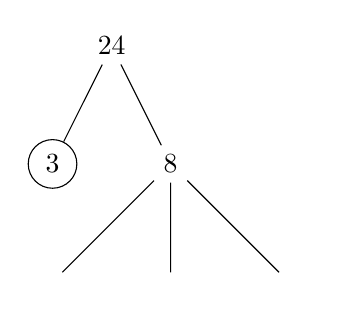
\begin{tikzpicture}[every node/level 1/.style={sibling distance=30mm},level 2/.style={sibling distance=15mm} ,
	circled/.style={draw, circle}
	]
	\node  {24}
	child {node [circled] {3}}
	child {node{8}
		child {node   {$\quad$ }}
		child {node   {$\quad$ }}
		child {node   {$\quad$ }
		}
	};
\end{tikzpicture} 
}\hfill 
	\parbox[position=t]{0.30\linewidth}{
	\begin{tikzpicture}[every node/level 1/.style={sibling distance=30mm},level 2/.style={sibling distance=15mm} ,
		circled/.style={draw, circle}
		]
		\node  {24}
		child {node [circled] {2}}
		child {node{12}
			child {node   {$\quad$ }}
			child {node {$\quad$ }
				child {node   {$\quad$ }}
				child {node { $\quad$} 
				}
			}
		};
	\end{tikzpicture} 
}
\end{example}
\begin{exercise}[sans calculatrice] Décomposer les nombres suivants en facteurs premiers.  
	\begin{multicols}{5}
		\begin{enumerate}[label={$\alph*=$}]
			\item $240$
			\item $18$ 
			\item $180$
			\item $90$
			\item $360$
			%			\item $60$
%			\item $950$
%			\item $24$
%			\item $12$
%			\item $144$
%			\item $89$
%			\item $93$
		\end{enumerate}
	\end{multicols}
\end{exercise}	
\begin{exercise}\hfill  

\noindent\parbox{0.40\linewidth}{
\begin{scratch}[scale=0.95,num blocks=true,print, fill blocks, fill gray=0.95] 
	%\blockinit{quand \greenflag est cliqué} 
	\blocksensing{demander \ovalnum{saisir un entier} et attendre}
	\blockvariable{mettre \selectmenu{N} à \ovalsensing{réponse}}
	\blockvariable{mettre \selectmenu{nbr} à \ovalnum{2}}
	\blockrepeat{répéter jusqu'à ce que \booloperator{\ovalvariable{N}  = \ovalnum{1} }  }
	{
		\blockifelse{si \booloperator{ \ovaloperator{\ovalvariable{N} modulo \ovalvariable{nbr}} = \ovalnum{0}}}
		{ 
			\blocklook{dire \ovalvariable{nbr} pendant \ovalnum{$5$} secondes} 
			\blockvariable{mettre \selectmenu{N} à \ovaloperator{\ovalvariable{N} / \ovalvariable{nbr}}}
		}
		{
			\blockvariable{ajouter \ovalnum{1} à \selectmenu{nbr}}
		}
	} 
\end{scratch} 
}\hfill 
\parbox{0.55\linewidth}{
\begin{enumerate}[label=\alph*), leftmargin=*]
	\item On saisit le nombre $150$. Lancer le script à la main.
	
Représenter le déroulement de l'algorithme en notant dans la colonne de droite les valeurs affichées par la ligne 6, et dans la colonne de gauche les valeurs successives de \ovalvariable{N} à la ligne 7.
	
		\Decomposition[TableauVerticalVide]{150}
		\Decomposition[TableauVerticalVide]{24}
		\item Même question si on saisit $24$.
		\item Quel est l'objet de cet algorithme ?
		\item Représenter le déroulement de l'algorithme pour \ovalvariable{N}=$2450$, $999$, $1122$ et $909$ :
\end{enumerate}
} 	 

\noindent\parbox{0.25\linewidth}{
\small\Decomposition[TableauVerticalVide]{2450} 
}\parbox{0.25\linewidth}{
\Decomposition[TableauVerticalVide]{1122}
}\parbox{0.25\linewidth}{
\Decomposition[TableauVerticalVide]{999}
} \parbox{0.25\linewidth}{
\Decomposition[TableauVerticalVide]{909}
} 
\end{exercise} 
\begin{example}\hfill 
	
\noindent\QCM[VF,Alterne,Stretch=1.1, Largeur=0.75cm]{%
	{$7$ est un facteur de $2\times 3^5\times 7^2$}&1,%
	{$6$ est un diviseur de $2\times 3^5\times 7^2$}&1,%
	{$14$ est un facteur de $2\times 3^5\times 7^2$}&1,%
	{$14$ est un facteur premier de $2\times 3^5\times 7^2$}&2,%
	{$11$ est un facteur premier de $2\times 3^5\times 7^2$}&2,%
	{$2\times 3^2$ est un facteur de $2\times 3^5\times 7^2$}&1,%
	{$ 3^4\times 7$ est un facteur de $2\times 3^5\times 7^2$}&1,%
	{$2\times 3^5\times 7^2$ est un multiple de $ 3^4\times 7$}&1,%
	{$2^2\times 3\times 7$ est un multiple de $2\times 3^5\times 7^2$}&2,% 
	{$2^6\times 3^8\times 11$ est un multiple de $2\times 3^5\times 7^2$}&2,%  
}
\end{example}   
\begin{exercise}\hfill 
	\begin{enumerate}[label=\alph*), leftmargin=*]
		\item À l'aide de la calculatrice donner la décomposition en facteurs premiers de $2520$.
		\item Entourer, sans calcul supplémentaire, les nombres qui divisent $2250$ : 
		\setlength{\abovedisplayskip}{5pt}
		\setlength{\belowdisplayskip}{5pt}
		\[
		13 \qquad 3\times 5\times 7 \qquad 2^2\times 3^2\times 5 \qquad 2^4\times 3
		\]
	\end{enumerate}
\end{exercise}
\begin{exercise}\hfill 
	\begin{enumerate}[label=\alph*), leftmargin=*]
		\item À l'aide de la calculatrice donner la décomposition en facteurs premiers de $1125$ et $450$.
		\item Entourer, sans calcul supplémentaire, les nombres qui sont des diviseurs communs à $1125$ et $450$ : 
		\setlength{\abovedisplayskip}{5pt}
		\setlength{\belowdisplayskip}{5pt}
		\[
		3\times 5 \qquad 3^2\times 5^4 \qquad 3\times 5^2\qquad 2\times 5^2\qquad 3^2\times 5 \qquad 3\times 5 \times 11
		\]
		\item Quel est la décomposition en facteur premier du plus grand diviseurs commun à $1125$ et $450$ ?
	\end{enumerate}
\end{exercise} 
\begin{exercise}\hfill 
\begin{enumerate}[label=\alph*), leftmargin=*]
	\item À l'aide de la calculatrice donner la décomposition en facteurs premiers de $360$.
	\item Entourer, sans calcul supplémentaire, les nombres qui sont des multiples de $360$ : 
	\setlength{\abovedisplayskip}{5pt}
	\setlength{\belowdisplayskip}{5pt}
	\[
	3^2\times 5\qquad 2^3\times 3^2\times 5^2 \qquad 2^4\times 5 \qquad 2^4\times 3^2\times 5\times 7
	\]
\end{enumerate}
\end{exercise}
\begin{exercise}\hfill 
	\begin{enumerate}[label=\alph*), leftmargin=*]
		\item À l'aide de la calculatrice donner la décomposition en facteurs premiers de $42$ et $70$.
		\item Entourer, sans calcul supplémentaire, les nombres qui sont des multiples communs à $42$ et $70$ : 
		\setlength{\abovedisplayskip}{5pt}
		\setlength{\belowdisplayskip}{5pt}
		\[
		2\times 3\times 7 \qquad 2\times 3\times 5\times 7\times 11 \qquad 2^2\times 5^2\qquad 2^3\times 3\times 5^2\times 7 \qquad 2^5\times 3\times 5^3 \qquad 2\times 3\times 5\times 7^2
		\]
		\item Quel est la décomposition en facteurs premiers du plus petit multiple commun à $1125$ et $450$ ?
	\end{enumerate}
\end{exercise}

   \begin{exercise}  \hfill 
   	
\noindent Un groupe d'élèves participent à une course d'orientation. On peut répartir les élèves présents en des équipes de 6, ou par équipes de 15, ou encore par équipes de 18.
   	
 Quel est le nombre minimum d'élèves présents ?
   \end{exercise}  
%----------------------------------------------------------------------------------------
%	 
%----------------------------------------------------------------------------------------
\cleardoublepage
\end{document}



